\section{Dependency Management}
Una delle parti più importanti di uno strumento di questo tipo è la gestione delle dipendenze che si divide in 2 parti: incoming files e outgoing files. Gradle ha bisogno di conoscere di cosa il nostro progetto ha bisogno per poter essere compilato ed eseguito le così dette dipendenze (dipendencies) che in questo caso sono gli incoming files. Gli outgoing files sono invece tutto ciò che il progetto produce, definite pubblicazioni (pubblications). Le dipendenze vengono specificate in forma di modules, è quindi necessario indicare dove si trovano questi modules in modo tale che Gradle li possa scaricare e impostare per il progetto che stiamo sviluppando. La posizione dove è possibile trovare i modules è definita repository, è necessario quindi dichiarare le repositories usate per le dipendenze volute. Ci sono 2 tipi di repository: 
\begin{enumerate}
    \item esterne, in questo caso la repository si trova in un server online adibito alla raccolta di modules
    \item interne, la repository è una cartella locale al progetto
\end{enumerate}
Per quanto riguarda quelle esterne Gradle si occuperà di scaricarle. E' possibile che alcune dipendenze vengano usate in più progetti, gradle mantiene quindi una cache locale, chiamata dependency cache, in cui salverà i modules già scaricati in modo da evitare di effettuare il download ad ogni build. Possiamo quindi immaginare che il ciclo di risoluzione delle dipendenze esterne sarà questo:
\begin{enumerate}
    \item ricerca delle dipendenze esterne nella cache locale
    \item se non si trovano nella cache locale si controlla se esistono nelle repository specificate
    \item se sono state trovate, vengono scaricate e inserite nella cache locale
\end{enumerate}
Nell'immagine è possibile vedere il percorso specifico che effettua la dependency resolution di Gradle:
\begin{figure}[H]
\centering
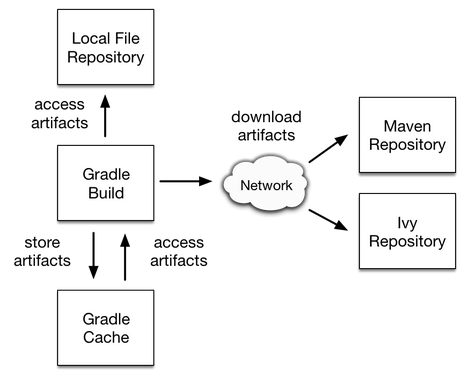
\includegraphics[width=0.4\linewidth]{HowToUse/3DependencyManagement/depMan.png}
\end{figure}
Analizziamo ora il caso di un progetto java.

\subsection{Dichiarazione delle dipendenze}
Prima di tutto è necessario indicare in che linguaggio il nostro progetto viene rilasciato (consideriamo d'ora in poi solo il caso di Java), per farlo aggiungiamo in testa al file build.gradle:
\begin{verbatim}
apply plugin: 'java' \end{verbatim}
A questo punto per poter usufruire di una dipendenza è necessario specificare da dove Gradle deve andare a prenderla, dobbiamo quindi indicare il repository remoto di riferimento. Se per esempio vogliamo che il nostro repository di riferimento sia Maven allora dobbiamo aggiungere al build.gradle:
\begin{verbatim}
repositories {
    mavenCentral()
} \end{verbatim}
In questo modo tutte le dipendenze che andremo a indicare successivamente saranno riferimenti alle pubblicazioni su Maven Central. La dichiarazione delle dipendenze deve essere inserita nel tag \texttt{dependencies} nel build.gradle file. Per esempio vogliamo avere junit 4.12 come dipendenza al nostro progetto Gradle allora dobbiamo aggiungere:
\begin{verbatim}
dependencies {
    testCompile group: 'junit', name: 'junit', version: '4.12' 
} \end{verbatim}
Osserviamo che nella dichiarazione ci sono 4 diversi indicatori:
\begin{itemize}
    \item \texttt{testCompile} indica lo scopo della dipendenza, in questo caso sarà importata durante la compilazione dei test;
    \item \texttt{group, name, version} corrispondono rispettivamente al groupId (nome del team o della società che ha sviluppato il modulo), artifactId (nome effettivo del modulo) e al version (versione del modulo) definiti su Maven.
\end{itemize}
Esiste un modo molto più diretto per indicare una dipendenza:
\begin{verbatim}
dependencies {
    testCompile 'junit:junit:4.12'
} \end{verbatim}
Ha lo stesso significato precedente ma ha una forma più compatta, forma che adotta anche la documentazione Maven.
\begin{figure}[H]
\centering
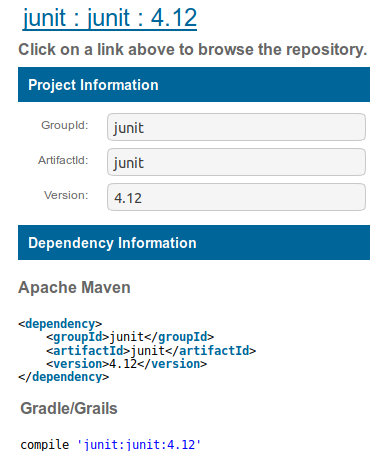
\includegraphics[width=0.4\linewidth]{HowToUse/3DependencyManagement/javaDep/gradleInMavenRepo.png}
\end{figure} 
Possiamo notare ora la differenza sostanziale della configurazione delle dipendenze tra il pom.xml di Maven e la build.gradle di Gradle. A questo punto per scaricare le dipendenze si deve eseguire il comando \texttt{dependencies} il cui output restituirà una lista di tutti i task con le relative dipendenze associate.